\section{Evidencia Experimental}

La Figura \ref{fig:ejecucion_openmp} presenta una ejecución de muestra de la implementación OpenMP durante los experimentos realizados.

\begin{figure}[H]
\centering
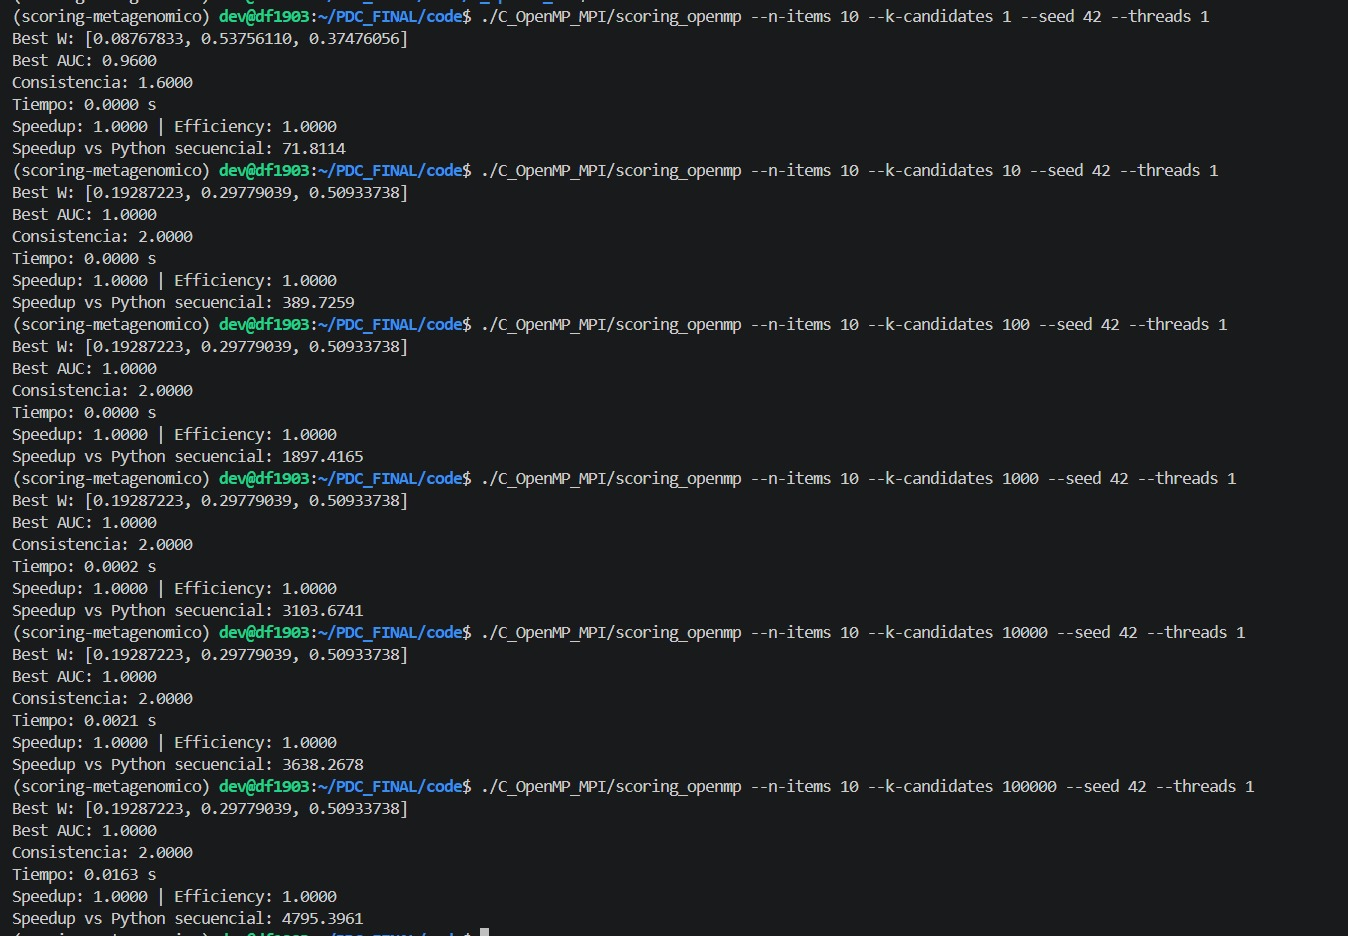
\includegraphics[width=.95\textwidth, height=0.45\textheight, keepaspectratio]
{figuras/capturas/openmp.png}
\caption{Ejecución de muestra de la implementación OpenMP.}
\label{fig:ejecucion_openmp}
\end{figure}

\subsection*{Pruebas con 1 hilo}

Las Figuras \ref{fig:openmp_1t_10} a \ref{fig:openmp_1t_50} presentan los resultados obtenidos utilizando 1 hilo con distinto número de ítems metagenómicos.

\begin{figure}[H]
\centering
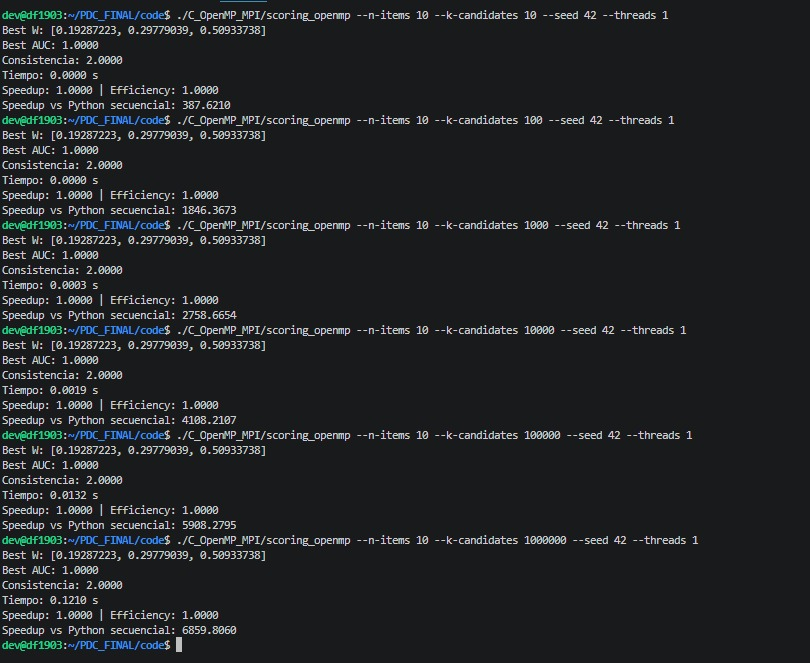
\includegraphics[width=.95\textwidth, height=0.45\textheight, keepaspectratio]
{figuras/capturas/openmp_1t_10.png}
\caption{OpenMP -- 1 hilo -- 10 ítems metagenómicos.}
\label{fig:openmp_1t_10}
\end{figure}

\begin{figure}[H]
\centering
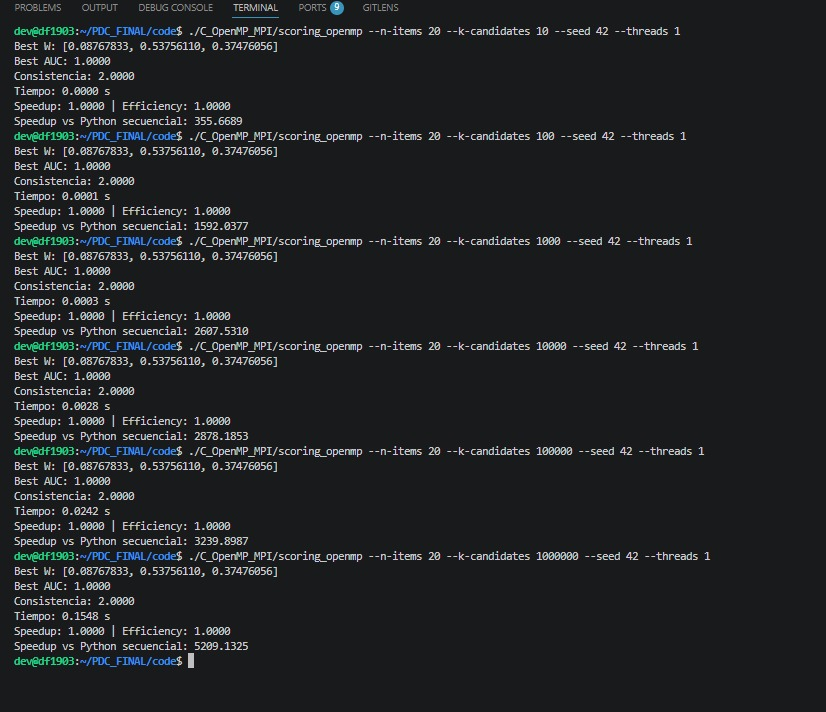
\includegraphics[width=.95\textwidth, height=0.45\textheight, keepaspectratio]
{figuras/capturas/openmp_1t_20.png}
\caption{OpenMP -- 1 hilo -- 20 ítems metagenómicos.}
\label{fig:openmp_1t_20}
\end{figure}

\begin{figure}[H]
\centering
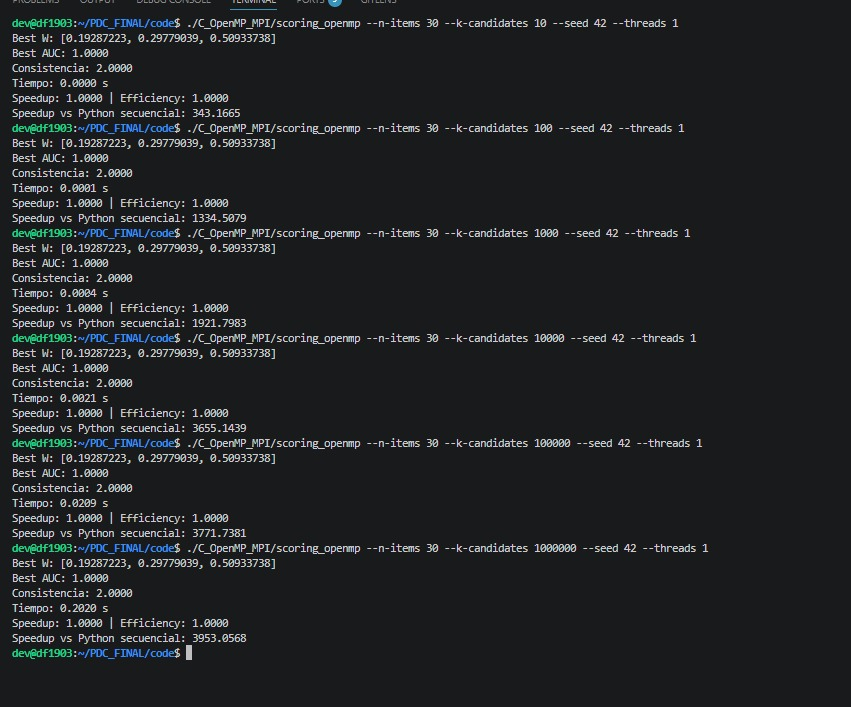
\includegraphics[width=.95\textwidth, height=0.45\textheight, keepaspectratio]
{figuras/capturas/openmp_1t_30.png}
\caption{OpenMP -- 1 hilo -- 30 ítems metagenómicos.}
\label{fig:openmp_1t_30}
\end{figure}

\begin{figure}[H]
\centering
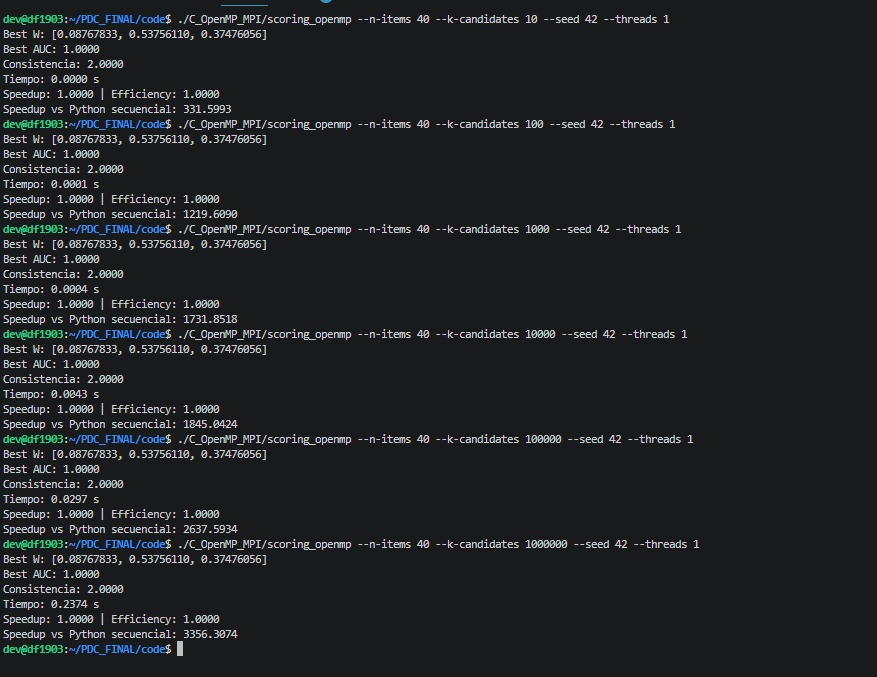
\includegraphics[width=.95\textwidth, height=0.45\textheight, keepaspectratio]
{figuras/capturas/openmp_1t_40.png}
\caption{OpenMP -- 1 hilo -- 40 ítems metagenómicos.}
\label{fig:openmp_1t_40}
\end{figure}

\begin{figure}[H]
\centering
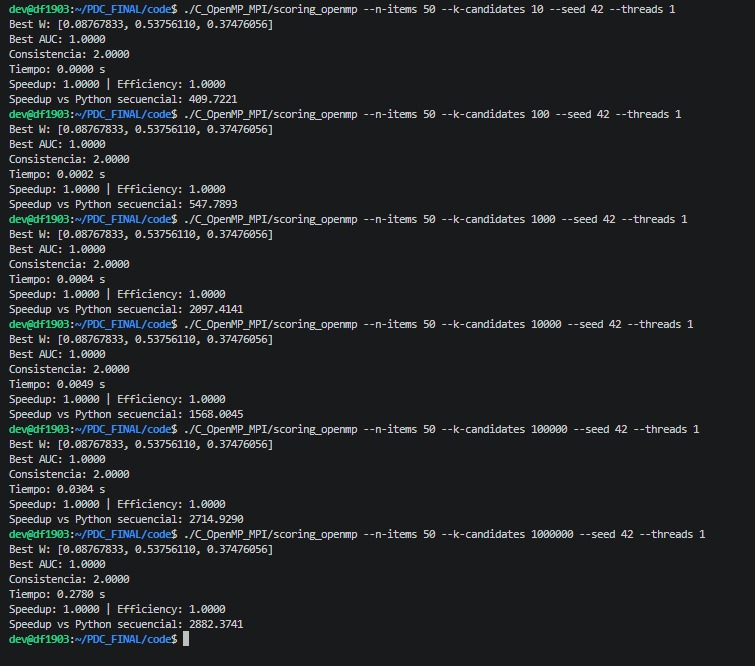
\includegraphics[width=.95\textwidth, height=0.45\textheight, keepaspectratio]
{figuras/capturas/openmp_1t_50.png}
\caption{OpenMP -- 1 hilo -- 50 ítems metagenómicos.}
\label{fig:openmp_1t_50}
\end{figure}

\subsection*{Pruebas con 2 hilos}

Las Figuras \ref{fig:openmp_2t_10} a \ref{fig:openmp_2t_50} presentan los resultados obtenidos utilizando 2 hilos con distinto número de ítems metagenómicos.

\begin{figure}[H]
\centering
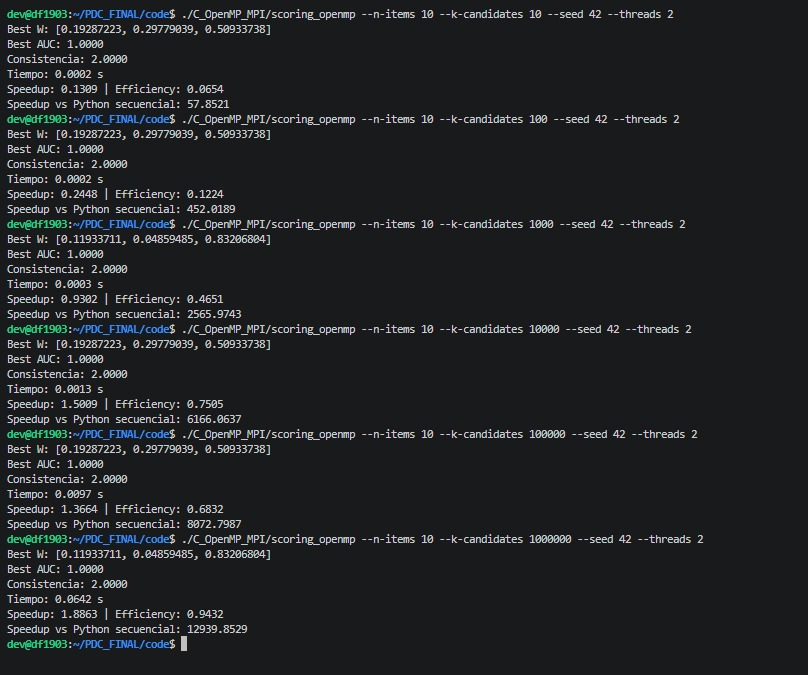
\includegraphics[width=.95\textwidth, height=0.45\textheight, keepaspectratio]
{figuras/capturas/openmp_2t_10.png}
\caption{OpenMP -- 2 hilos -- 10 ítems metagenómicos.}
\label{fig:openmp_2t_10}
\end{figure}

\begin{figure}[H]
\centering
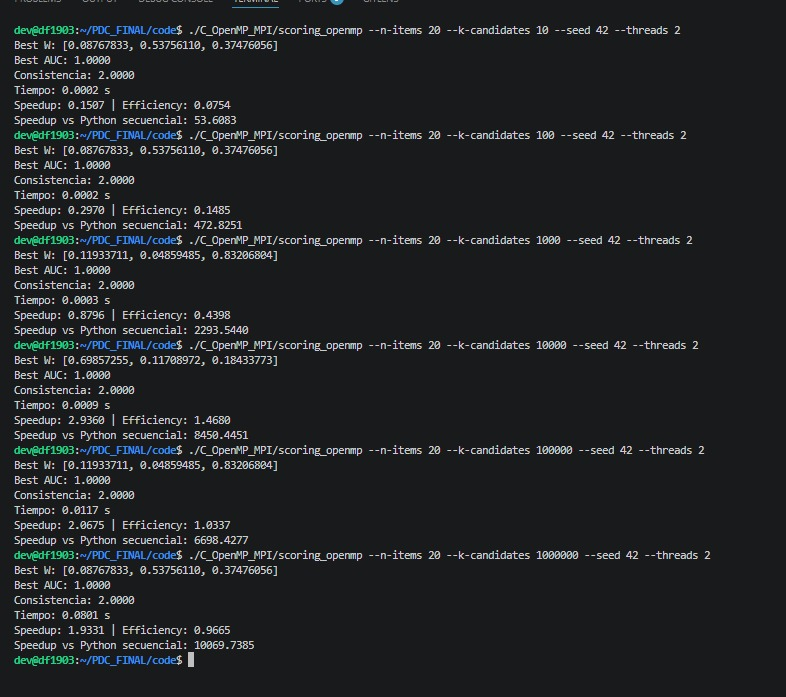
\includegraphics[width=.95\textwidth, height=0.45\textheight, keepaspectratio]
{figuras/capturas/openmp_2t_20.png}
\caption{OpenMP -- 2 hilos -- 20 ítems metagenómicos.}
\label{fig:openmp_2t_20}
\end{figure}
Durante cada prueba se registró automáticamente el tiempo total de procesamiento, el mejor valor de ROC-AUC encontrado y la información correspondiente a los hilos utilizados.